% outline

% Intro
% Brief history
% Why?
% goto with settrace
% goto with bytecodes
% Crashing python with bytescodes
% Problems...
% Performance!

\documentclass{beamer}
\usepackage{minted}
\usetheme{default}
\hypersetup{colorlinks=true}
\usepackage{framed}
\usepackage[normalem]{ulem}
\usepackage{color}
\usepackage{graphicx}

\title{goto in Python 3. Yes. Really.}
\subtitle{Kiwi PyCon 2014}
\author{\texorpdfstring{Carl Cerecke\newline\url{carl@free.org.nz}}{Carl Cerecke}}
%\address{carl\@free.org.nz}
\institute{https://github.com/cdjc/goto}
\date{September 13-14, 2014}

\begin{document}

    \begin{frame}[plain]
        \titlepage
    \end{frame}

\begin{frame}[fragile]{BASIC on the Commodore 64}
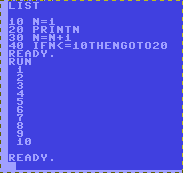
\includegraphics{c64.png}
\end{frame}

\begin{frame}{History}

\begin{itemize}
\item In the beginning was the \texttt{goto}
\item 1958 Heinz Zemanek expresses doubts about goto at pre-ALGOL meeting.
\item 1968 Edsgar Dijkstra ``GOTO Considered Harmful''
\item 1974 Don Knuth ``Structured Programming with go to statements''
\item 1987 Frank Rubin ` ``GOTO Considered Harmful'' Considered Harmful'
\end{itemize}

\end{frame}

\begin{frame}{Why add goto to Python?}

It seemed like a good idea at the time...
\vspace{1cm}

Also useful for:
\begin{itemize}
\item State machines
\item Breaking out of a nested loop
\item Generating python code programmatically
\item Translating goto-filled code to python
\end{itemize}

\end{frame}

\begin{frame}{But it's already been done before!}

\begin{itemize}
\item April 1 2004, \href{http://entrian/goto}{http://entrian/goto}

\item Uses \texttt{sys.settrace}

\item Checks before the execution of \emph{every line} for goto. Slow

\item Module scope, not function scope.
\end{itemize}
\end{frame}

\begin{frame}[fragile]{Goto using bytecode manipulation}

\begin{itemize}
\item Python bytecodes already have gotos:
\item JUMP\_FORWARD(delta)
\item JUMP\_ABSOLUTE(target)
\item also exotics like JUMP\_IF\_FALSE\_OR\_POP(target)
\end{itemize}

\end{frame}

\begin{frame}[fragile]{Simple example function}



\begin{minted}{python}
from goto import goto

@goto            # enables goto in decorated function
def simple(n):
    goto .skip
    print(n)
    label .skip
\end{minted}

We can see python bytecodes:

\begin{minted}{python}
import dis
dis.dis(fn)      # pretty print byte code
\end{minted}

\end{frame}

\begin{frame}[fragile]{Disassembly of simple function (without goto decorator)}
\begin{tabular}{l|r|l|r|l}
line & addr & opcode & par & interpretation \\
\hline
302 &          0 & LOAD\_GLOBAL         &     0 & (goto)  \\
     &           3 &  LOAD\_ATTR               &   1  & (skip)  \\
      &          6 &  POP\_TOP      &  &           \\
\hline
303   &          7 &  LOAD\_GLOBAL         &       2  & (print)  \\
          &     10 &  LOAD\_FAST           &       0 &  (n)  \\
              & 13 &  CALL\_FUNCTION        &      1  & (1 positional, 0 keyword pair)  \\
     &          16 &  POP\_TOP            &     &  \\
\hline
304   &         17 &  LOAD\_GLOBAL        &        3  & (label)  \\
     &          20 &  LOAD\_ATTR          &        1  & (skip)  \\
     &          23 &  POP\_TOP            &     &  \\
\hline     
     &          24 &  LOAD\_CONST         &        0  & (None)  \\
     &          27 &  RETURN\_VALUE      &      &  \\
\end{tabular}
\end{frame}

\begin{frame}[fragile]{Changes required for goto}

\begin{itemize}
\item Python treats \verb!goto! statement as attribute access.
\item Likewise for \verb!label! statement.

\item Need to change \verb!goto! into \verb!JUMP_ABSOLUTE!

\item and \verb!label! into \verb!NOP!
\end{itemize}
\end{frame}

\begin{frame}[fragile]{Byte code with goto changes}
\begin{tabular}{l|r|l|r|l}
line & addr & opcode & par & interpretation \\
\hline
302 &          0 & \textcolor{red}{JUMP\_ABSOLUTE}         &     24 &  \\
     &           3 &  \sout{LOAD\_ATTR}               &   1  & (skip)  \\
      &          6 &  \sout{POP\_TOP}      &  &           \\
\hline
303   &          7 &  LOAD\_GLOBAL         &       2  & (print)  \\
          &     10 &  LOAD\_FAST           &       0 &  (n)  \\
              & 13 &  CALL\_FUNCTION        &      1  & (1 positional, 0 keyword pair)  \\
     &          16 &  POP\_TOP            &     &  \\
\hline
304   &         17 &  \textcolor{red}{NOP}        &          &   \\
      &         18 &  \textcolor{red}{NOP}        &          &   \\
      &         19 &  \textcolor{red}{NOP}        &          &   \\
      &         20 &  \textcolor{red}{NOP}        &          &   \\
      &         21 &  \textcolor{red}{NOP}        &          &   \\
      &         22 &  \textcolor{red}{NOP}        &          &   \\
      &         23 &  \textcolor{red}{NOP}        &          &   \\
\hline
target     &          24 &  LOAD\_CONST         &        0  & (None)  \\
     &          27 &  RETURN\_VALUE      &      &  \\
\end{tabular}
\end{frame}

\begin{frame}[fragile]{How to change bytecodes?}
Decorator outline (code at \href{http://github.com/cdjc/goto} {http://github.com/cdjc/goto} )
\begin{itemize}
\item \verb!c = fn.__code__  #! code object. Not read only :-)
\item \verb!c.co_code        #! bytecode string. Read only :-(
\item Find all labels and gotos in \verb!c.co_code!
\item \verb!NOP! all labels.
\item Make gotos into \verb!JUMP_ABSOLUTE!
\item Make new code object
\item \verb!fn.__code__! = new code object
\item \verb!return fn!
\end{itemize}
\end{frame}

\begin{frame}[fragile]{Problems!}
\begin{minted}{python}
    @goto
    def infinite(n):
        label .start
        for i in 'oops':
            goto .start
\end{minted}

\begin{itemize}
\item At loop-start, python adds a 'block'.
\item At loop-end python does \verb!POP_BLOCK!
\item Jumping out of a loop must \verb!POP_BLOCK! before jump.
\item Illegal:
\begin{itemize}
\item Jump into a loop (Segmentation Fault on \verb!POP_BLOCK!)
\item Jump into/out of \verb!try!, \verb!except!, \verb!finally!, \verb!with!
\item Multiple identical labels (or missing label)
\item Jump out of loop nested more than four deep.
\end{itemize}
\end{itemize}
\end{frame}

\begin{frame}[fragile]{Performance}
%\includepdf[pages={1}, fitpaper=false]{oddeven.pdf}
\includegraphics[scale=0.5]{oddeven.pdf}

\begin{itemize}
\item Function-based state machine within a class
\item Goto-based state machine within a function
\item \verb!while! loop in plain code
\end{itemize}

The \emph{even} state breaks at n = 100000000

Python 3.3.1 on Linux VM
\end{frame}

\begin{frame}[fragile]{Performance (function-based state machine)}

%Function-based state machine
\begin{minted}{python}
class state_machine:
    def even_state(self):
        ...
        return self.odd_state
    def odd_state(self):
        ...
        return self.even_state
    def go():
        state = self.even_state
        while state:
            state = state()
\end{minted}
\alert{35.0 seconds}
\end{frame}


\begin{frame}[fragile]{Performance (plain while loop)}
\begin{minted}{python}
n = 0
while n != limit:
    n += 1         # even -> odd
    n += 1         # odd -> even
\end{minted}
\alert{11.5 seconds}
\end{frame}

\begin{frame}[fragile]{Performance (goto-based state machine)}
%\vspace{-1cm}
\begin{minted}{python}
@goto
def goto_state_machine(limit):
    n = 0

    label .state_even  ### even_state
    if n == limit:
        return
    n += 1
    goto .state_odd
    ################
    label .state_odd   ### odd_state
    n += 1
    goto .state_even
\end{minted}
\pause
\alert{7.2 seconds!}  (over 4 seconds \emph{faster} than a \verb!while! loop!)

\pause
But... \verb!while! loop \emph{inside} function: \alert{7.1 seconds.} :-(
\end{frame}

\begin{frame}[fragile]{Future work}

\begin{itemize}
\item Remove some restrictions where sensible.
\item pypi or something...
\item \verb!comefrom! statement
\item Computed \verb!goto!
\end{itemize}

\end{frame}

\end{document}
